%!TEX TS-program = xelatex
\documentclass[12pt, a4paper, oneside]{article}

% Можно вставить разную преамбулу
% пакеты для математики
\usepackage{amsmath,amsfonts,amssymb,amsthm,mathtools}  
\mathtoolsset{showonlyrefs=true}  % Показывать номера только у тех формул, на которые есть \eqref{} в тексте.

\usepackage[british,russian]{babel} % выбор языка для документа
\usepackage[utf8]{inputenc}          % utf8 кодировка

% Основные шрифты 
\usepackage{fontspec}         
\setmainfont{Linux Libertine O}  % задаёт основной шрифт документа

% Математические шрифты 
\usepackage{unicode-math}     
\setmathfont[math-style=upright]{euler.otf} 

\setmathfont[range={\mathbb, \mathop, \heartsuit, \angle, \smile, \varheartsuit}]{Asana-Math.otf}

%%%%%%%%%% Работа с картинками и таблицами %%%%%%%%%%
\usepackage{graphicx} % Для вставки рисунков                
\usepackage{graphics}
\graphicspath{{images/}{pictures/}}   % папки с картинками

\usepackage[figurename=Картинка]{caption}

\usepackage{wrapfig}    % обтекание рисунков и таблиц текстом

\usepackage{booktabs}   % таблицы как в годных книгах
\usepackage{tabularx}   % новые типы колонок
\usepackage{tabulary}   % и ещё новые типы колонок
\usepackage{float}      % возможность позиционировать объекты в нужном месте
\renewcommand{\arraystretch}{1.2}  % больше расстояние между строками


%%%%%%%%%% Графики и рисование %%%%%%%%%%
\usepackage{tikz, pgfplots}  % языки для графики
%\pgfplotsset{compat=1.16}

\usepackage{todonotes} % для вставки в документ заметок о том, что осталось сделать
% \todo{Здесь надо коэффициенты исправить}
% \missingfigure{Здесь будет Последний день Помпеи}
% \listoftodos --- печатает все поставленные \todo'шки

\usepackage{multicol}

%%%%%%%%%% Внешний вид страницы %%%%%%%%%%

\usepackage[paper=a4paper, top=20mm, bottom=15mm,left=20mm,right=15mm]{geometry}
\usepackage{indentfirst}    % установка отступа в первом абзаце главы

\usepackage{setspace}
\setstretch{1.15}  % межстрочный интервал
\setlength{\parskip}{4mm}   % Расстояние между абзацами
% Разные длины в LaTeX: https://en.wikibooks.org/wiki/LaTeX/Lengths

% свешиваем пунктуацию
% теперь знаки пунктуации могут вылезать за правую границу текста, при этом текст выглядит ровнее
\usepackage{microtype}

% \flushbottom                            % Эта команда заставляет LaTeX чуть растягивать строки, чтобы получить идеально прямоугольную страницу
\righthyphenmin=2                       % Разрешение переноса двух и более символов
\widowpenalty=300                     % Небольшое наказание за вдовствующую строку (одна строка абзаца на этой странице, остальное --- на следующей)
\clubpenalty=3000                     % Приличное наказание за сиротствующую строку (омерзительно висящая одинокая строка в начале страницы)
\tolerance=10000     % Ещё какое-то наказание.

% мои цвета https://www.artlebedev.ru/colors/
\definecolor{titleblue}{rgb}{0.2,0.4,0.6} 
\definecolor{blue}{rgb}{0.2,0.4,0.6} 
%\definecolor{red}{rgb}{1,0,0.2} 
\definecolor{green}{rgb}{0, 0.6, 0}
\definecolor{purp}{rgb}{0.4,0,0.8} 

\definecolor{red}{RGB}{213,94,0}
\definecolor{yellow}{RGB}{240,228,66}


% цвета из geogebra 
\definecolor{litebrown}{rgb}{0.6,0.2,0}
\definecolor{darkbrown}{rgb}{0.75,0.75,0.75}

% Гиперссылки
\usepackage{xcolor}   % разные цвета

\usepackage{hyperref}
\hypersetup{
	unicode=true,           % позволяет использовать юникодные символы
	colorlinks=true,       	% true - цветные ссылки
	urlcolor=blue,          % цвет ссылки на url
	linkcolor=black,          % внутренние ссылки
	citecolor=green,        % на библиографию
	breaklinks              % если ссылка не умещается в одну строку, разбивать её на две части?
}

% меняю оформление секций 
\usepackage{titlesec}
\usepackage{sectsty}

% меняю цвет на синий
\sectionfont{\color{titleblue}}
\subsectionfont{\color{titleblue}}

% кружочки у цифр в секциях
\renewcommand{\thesection}{\arabic{section}}

% https://ru.overleaf.com/learn/latex/Sections_and_chapters

% выбрасываю нумерацию страниц и колонтитулы 
%\pagestyle{empty}

% синие круглые бульпоинты в списках itemize 
\usepackage{enumitem}

\definecolor{itemizeblue}{rgb}{0, 0.45, 0.70}

\newcommand*{\MyPoint}{\tikz \draw [baseline, fill=itemizeblue, draw=blue] circle (2.5pt);}
\renewcommand{\labelitemi}{\MyPoint}

\AddEnumerateCounter{\asbuk}{\@asbuk}{\cyrm}
\renewcommand{\theenumi}{\asbuk{enumi}}

% расстояние в списках
\setlist[itemize]{parsep=0.4em,itemsep=0em,topsep=0ex}
\setlist[enumerate]{parsep=0.4em,itemsep=0em,topsep=0ex}

% эпиграфы
\usepackage{epigraph}
\setlength\epigraphwidth{.6\textwidth}
\setlength\epigraphrule{0pt}

%%%%%%%%%% Свои команды %%%%%%%%%%

% Математические операторы первой необходимости:
\DeclareMathOperator{\sgn}{sign}
\DeclareMathOperator*{\argmin}{arg\,min}
\DeclareMathOperator*{\argmax}{arg\,max}
\DeclareMathOperator{\Cov}{Cov}
\DeclareMathOperator{\Var}{Var}
\DeclareMathOperator{\Corr}{Corr}

\DeclareMathOperator{\Pois}{Pois}
\DeclareMathOperator{\Geom}{Geom}
\DeclareMathOperator{\Exp}{Exp}

%\DeclareMathOperator{\E}{\mathbb{E}}
\DeclareMathOperator{\Med}{Med}
\DeclareMathOperator{\Mod}{Mod}
\DeclareMathOperator*{\plim}{plim}

% команды пореже
\newcommand{\const}{\mathrm{const}}  % const прямым начертанием
\newcommand{\iid}{\sim i\,i\,d\,\,}  % ну вы поняли...
\newcommand{\fr}[2]{\ensuremath{^{#1}/_{#2}}}   % особая дробь
\newcommand{\ind}[1]{\mathbbm{1}_{\{#1\}}} % Индикатор события
\newcommand{\dx}[1]{\,\mathrm{d}#1} % для интеграла: маленький отступ и прямая d

% одеваем шапки на частые штуки
\def \hb{\hat{\beta}}
\def \hs{\hat{s}}
\def \hy{\hat{y}}
\def \hY{\hat{Y}}
\def \he{\hat{\varepsilon}}
\def \hVar{\widehat{\Var}}
\def \hCorr{\widehat{\Corr}}
\def \hCov{\widehat{\Cov}}

% Греческие буквы
\def \a{\alpha}
\def \b{\beta}
\def \t{\tau}
\def \dt{\delta}
\def \e{\varepsilon}
\def \ga{\gamma}
\def \kp{\varkappa}
\def \la{\lambda}
\def \sg{\sigma}
\def \tt{\theta}
\def \Dt{\Delta}
\def \La{\Lambda}
\def \Sg{\Sigma}
\def \Tt{\Theta}
\def \Om{\Omega}
\def \om{\omega}

% Готика
\def \mA{\mathcal{A}}
\def \mB{\mathcal{B}}
\def \mC{\mathcal{C}}
\def \mE{\mathcal{E}}
\def \mF{\mathcal{F}}
\def \mH{\mathcal{H}}
\def \mL{\mathcal{L}}
\def \mN{\mathcal{N}}
\def \mU{\mathcal{U}}
\def \mV{\mathcal{V}}
\def \mW{\mathcal{W}}

% Жирные буквы
\def \mbb{\mathbb}
\def \RR{\mbb R}
\def \NN{\mbb N}
\def \ZZ{\mbb Z}
\def \PP{\mbb{P}}
\def \E{\mbb{E}}
\def \QQ{\mbb Q}

\def\F{\ensuremath{\mathcal{F}}} % аналогично!

%%%%%%%%%% Теоремы %%%%%%%%%%
\theoremstyle{plain} % Это стиль по умолчанию.  Есть другие стили.
\newtheorem{theorem}{Теорема}[section]
\newtheorem{proposition}{Утверждение}[section]
\newtheorem{result}{Следствие}[section]

% убирает курсив и что-то еще наверное делает ;)
\theoremstyle{definition}         
\newtheorem*{definition}{Определение}  % нумерация не идёт вообще


%%%%%%%%%% Задачки и решения %%%%%%%%%%
\usepackage{etoolbox}    % логические операторы для своих макросов
\usepackage{environ}
\newtoggle{lecture}

\newcounter{probNum}[section]  % счётчик для упражнений 
\NewEnviron{problem}[1]{%
    \refstepcounter{probNum}% увеличели номер на 1 
    {\noindent \textbf{\large \color{titleblue} Упражнение~\theprobNum~#1}  \\ \\ \BODY}
    {}%
  }

% Окружение, чтобы можно было убирать решения из pdf
\NewEnviron{sol}{%
  \iftoggle{lecture}
    {\noindent \textbf{\large Решение:} \\ \\ \BODY}
    {}%
  }
 
% выделение по тексту важных вещей
\newcommand{\indef}[1]{\textbf{ \color{green} #1}} 

% разные дополнения для картинок
\usetikzlibrary{arrows.meta}
\usepackage{varwidth}

\usepackage[normalem]{ulem}  % для зачекивания текста

% Если переключить в false, все solution исчезнут из pdf
\toggletrue{lecture}
%\togglefalse{lecture}



\title{
\begin{center} 
\includegraphics[width=0.99\textwidth]{logo.png}
\end{center}
Гипотеза о равенстве средних и доверительные интервалы}
% Посиделка 4: распределение среднего}
\date{ } %\today}

\author{Ульянкин Ппилиф \thanks{\url{https://github.com/FUlyankin/matstat_lec}}}

\begin{document} % Конец преамбулы, начало файла

\maketitle

% \epigraph{Чтобы забыть что-нибудь ненужное, надо сначала выучить что-нибудь ненужное.}{\textit{Кот Матроскин про матстат}}

% В этой посиделке мы начнём строить статистику, основанную на средних. Мы примем на веру, что среднее имеет нормальное распределение, посчитаем его характеристики, построим доверительный интервал и проверим целую гипотезу.  

Поговорим про мощность различных процедур. Мы с вами обсудили, что гипотезу о равенстве средних можно проверить с помощью следующей процедуры. 

\subsection*{Процедура 1}

\begin{enumerate}
\item  Собираем выборки $X_1, \ldots, X_n$ и $Y_1, \ldots, Y_n$;
\item  Находим значение статистики

$$
z_{obs} = \frac{\bar x - \bar y}{\sqrt{\frac{s_x^2}{n_x} + \frac{s_y^2}{n_y}}};
$$

\item Говорим, что по ЦПТ $z_{obs} \overset{asy}{\sim} N(0,1);$
\item Находим критическое значение $z_{1 - \frac{\alpha}{2}}$;
\item Если мы видим, что $|z_{obs}| <  z_{1 - \frac{\alpha}{2}}$, мы говорим, что гипотеза не отвергается. 
\end{enumerate}

Ту же саму гипотезу можно попробовать проверить с помощью другого алгоритма, основанного на доверительных интервалах.

\newpage

\subsection*{Процедура 2}

\begin{enumerate}
\item  Собираем выборки $X_1, \ldots, X_n$ и $Y_1, \ldots, Y_n$;
\item  Находим $\bar x$ и $\bar y$;
\item  Пользуясь ЦПТ и зная, что $\bar x \overset{asy}{\sim} N \left(\mu_1,\frac{s^2_x}{n_x} \right)$ и $\bar y \overset{asy}{\sim} N\left(\mu_2,\frac{s^2_y}{n_y}\right)$ строим для $\mu_1$ и $\mu_2$ доверительные интервалы;
\item Если доверительные интервалы пересеклись, говорим, что гипотеза не отвергается. 
\end{enumerate}

Вроде бы вторая процедура выглядит довольно естественно, однако ей никто не пользуется. Дело в том, что для одинаковых ошибок первого рода, $\alpha$, ошибка второго рода, $\beta$, для процедуры, основанной на доверительных интервалах, окажется выше. Задание состоит в том, чтобы это увидеть.

Для простоты будем дальше предполагать, что $\bar x > \bar y$. Также будем считать, что обе дисперсии известны и равны единице, $\sigma^2_x = \sigma^2_y = 1$. Объёмы выборок одинаковы, $n_x = n_y = n$. Альтернатива односторонняя, то есть наблюдаемое значение статистики нужно искать как $z_{1 - \alpha}$. 


\subsection*{Решение}

Гипотеза о равенстве средних не отвергается, если

$$
\frac{\bar{x} - \bar{y}}{\sqrt{\frac{\sigma^2_x}{n_x} + \frac{\sigma^2_y}{n_y}}} < z_{1-\alpha}.
$$

Упростим выражение

$$
\frac{\bar{x} - \bar{y}}{\sqrt{\frac{2}{n}}} < z_{1-\alpha}.
$$

Найдём ошибку второго рода

\begin{multline*}
\mathbb{P} \left( H_0 \mid H_a \right) = \mathbb{P} \left( \frac{\bar{x} - \bar{y}}{\sqrt{\frac{2}{n}}} < z_{1-\alpha} \mid \mu_1 \ne \mu_2 \right)  = \\ = \mathbb{P} \left( \frac{\bar{x} - \bar{y} - (\mu_1 - \mu_2)}{\sqrt{\frac{2}{n}}} < z_{1-\alpha} - \frac{\mu_1 - \mu_2}{\sqrt{\frac{2}{n}}} \mid \mu_1 \ne \mu_2 \right) = \mathbb{P} \left( \mN(0,1) < z_{1-\alpha} - \frac{\mu_1 - \mu_2}{\sqrt{\frac{2}{n}}} \right) = \\ = \Phi \left( z_{1-\alpha} - \frac{\mu_1 - \mu_2}{\sqrt{\frac{2}{n}}} \right).
\end{multline*}


% def power_1(n_obs, alpha=0.05, mu1=4, mu2=5, sigma=1):
%     z_crit = stats.norm().ppf(1 - alpha)
%     a = z_crit - (mu2 - mu1)/np.sqrt(2 * sigma/n_obs)
%     return 1 - stats.norm().cdf(a)


Построим доверительные интервалы для средних:

$$
\begin{aligned} 
& \bar{x} \pm z_{1 - \alpha} \cdot \sqrt{ \frac{1}{n} } \\
& \bar{y} \pm z_{1 - \alpha} \cdot \sqrt{ \frac{1}{n} }
\end{aligned} 
$$

Если доверительные интервалы пересекаются, гипотеза не отвергается, то есть: 

$$
\begin{aligned} 
& \bar{x} - z_{1 - \alpha} \cdot \sqrt{ \frac{1}{n} } < \bar{y} + z_{1 - \alpha} \cdot \sqrt{ \frac{1}{n} } \\
& \bar{x} - \bar{y} < 2 \cdot z_{1 - \alpha} \cdot \sqrt{ \frac{1}{n} } \\
& \frac{\bar{x} - \bar{y}}{  \sqrt{ \frac{1}{n} } }  < 2 \cdot z_{1 - \alpha} \\
& \frac{\bar{x} - \bar{y}}{  \sqrt{ \frac{2}{n} } }  < \sqrt{2} \cdot z_{1 - \alpha} \\
\end{aligned} 
$$

Напомню, что для простоты мы считаем, что $\bar x > \bar y$. Найдём ошибку второго рода

\begin{multline*}
\mathbb{P} \left( H_0 \mid H_a \right)  = \mathbb{P} \left( \frac{\bar{x} - \bar{y} - (\mu_1 - \mu_2)}{\sqrt{\frac{2}{n}}} < \sqrt{2} \cdot z_{1-\alpha} - \frac{\mu_1 - \mu_2}{\sqrt{\frac{2}{n}}} \mid \mu_1 \ne \mu_2 \right) = \\ = \mathbb{P} \left( \mN(0,1) < \sqrt{2} \cdot z_{1-\alpha} - \frac{\mu_1 - \mu_2}{\sqrt{\frac{2}{n}}} \mid \mu_1 \ne \mu_2 \right) = \Phi \left( \sqrt{2} \cdot  z_{1-\alpha} - \frac{\mu_1 - \mu_2}{\sqrt{\frac{2}{n}}} \right).
\end{multline*}

% def power_2(n_obs, alpha=0.05, mu1=4, mu2=5, sigma=1):
%     z_crit = stats.norm().ppf(1 - alpha)
%     a = np.sqrt(2)*z_crit - (mu2 - mu1)/np.sqrt(2 * sigma**2/n_obs)
%     return 1 - stats.norm().cdf(a)

Чем больше наблюдений есть в нашем распоряжении, тем больше мощность теста. Нарисуем функции, описывающие мощность в координатах число наблюдений, мощность. На картинке видно, что первая процедура стабильно выигрывает у второй. При бесконечном числе наблюдений разницы не будет, так как мы всегда сможем идеально отделить две альтернативы друг от друга. 

\begin{center} 
    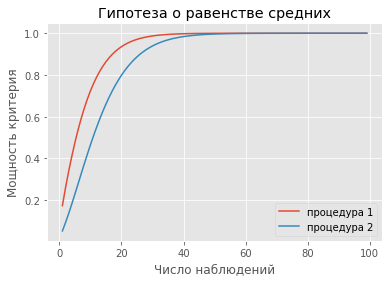
\includegraphics[width=0.8\linewidth]{eqmeqn.png}
\end{center} 





\end{document}
